
Following previous intuitive logic studies \citep[e.g.][]{Mevel2014}
I calculated the number of heuristic responses given
by each participant on conflict problems, 
and categorised each participant as either
``majority heuristic'' (3 or 4 heuristic responses out of four, 53 participants)
or ``minority heuristic'' (0 to 2 heuristic responses, 75 participants).
In this appendix, I repeat the time course analyses
reported for Experiment 6 separately for each group of participants.
As none of the trends differ qualitatively from the results
reported in Chapter 6 in ways that affect my conclusions,
I do not provide interpretation of each individual figure.


\begin{figure}[h]
  \centering
  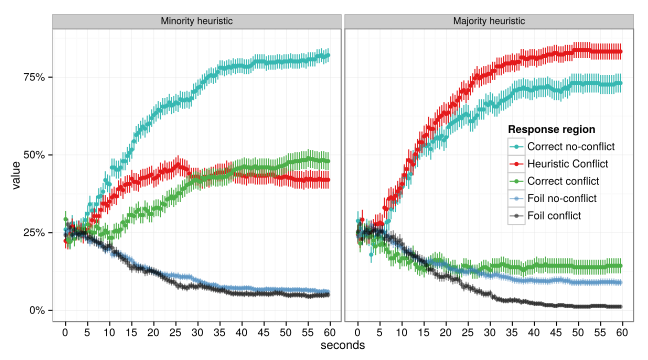
\includegraphics[width=.9\textwidth]{imgs/exp6/all_bias.pdf}
  %% \caption[Proportion of mouse cursors in each responses' region of the screen over time,
  %%   for minority heuristic and majority heuristic particiapants, 
  %%   Experiment 6.]{
  \caption[]{
    Proportion of mouse cursors in the region of the screen 
    corresponding to each response options, over time, 
    for conflict and no-conflict problems,
    separately for minority heuristic and majority heuristic participants
    (see also Figure~\ref{fig:exp6-all}).
  }
\end{figure}

\begin{figure}[h]
  \centering
  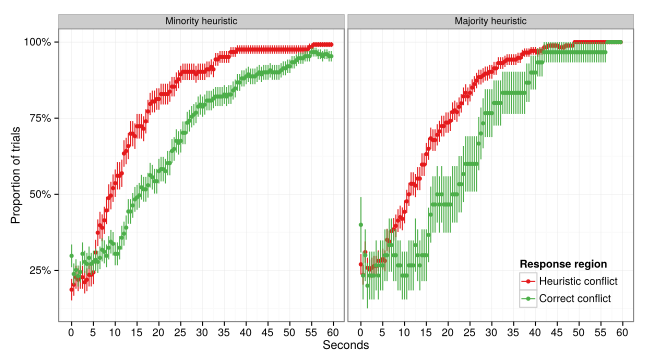
\includegraphics[width=.9\textwidth]{imgs/exp6/conflict-to-chosen_bias.pdf}
  %% \caption[Proportion of cursor in region of chosen response option
  %%   for minority heuristic and majority heuristic particiapants, 
  %%   Experiment 6.]{
  \caption[]{
    Proportion of mouse cursors in the region of
    the response option which was ultimately selected on that trial,
    comparing movements to the heuristic and correct options on conflict problems,
    separately for minority heuristic and majority heuristic participants
    (see also Figure~\ref{fig:exp6-all-to-chosen}).
  }
\end{figure}

\begin{figure}[h]
  \centering
  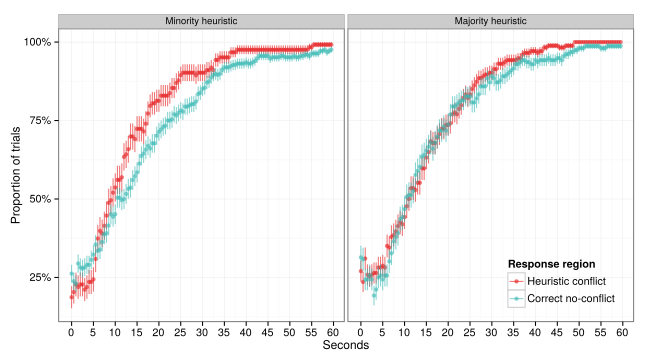
\includegraphics[width=.9\textwidth]{imgs/exp6/intuitive-to-chosen_bias.pdf}
  %% \caption[for minority heuristic and majority heuristic particiapants, 
  %%   Experiment 6.]{
  \caption[]{
    Proportion of mouse cursors in the region of
    the response option which was ultimately selected on that trial,
    comparing movements to the heuristic option conflict problems
    to those to the correct options on no-conflict problems,
    separately for minority heuristic and majority heuristic participants
    (see also Figure~\ref{fig:exp6-all-to-chosen}).
  }
\end{figure}

\begin{figure}[h]
  \centering
  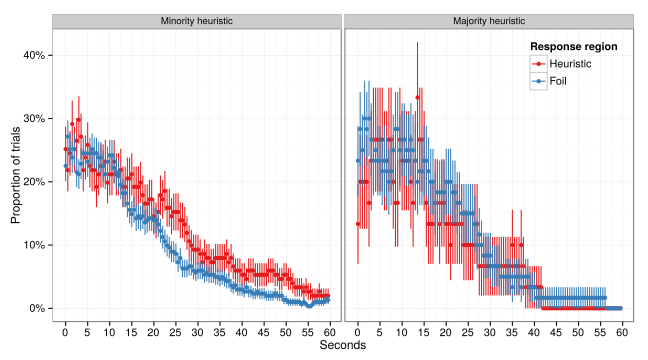
\includegraphics[width=.9\textwidth]{imgs/exp6/correct-not-chosen_bias.pdf}
  %% \caption[Proportion of cursor in region of other response options
  %%   when correct response was given
  %%   for minority heuristic and majority heuristic particiapants, 
  %%   Experiment 6.]{
  \caption[]{   
    Proportion of trials in the region of each option, over time,
    for trials in which the correct option was eventually chosen,
    separately for minority heuristic and majority heuristic participants
    (see also Figure~\ref{fig:exp6-correct-not-chosen}).
    Error bars show standard error of measurement.
  }
\end{figure}

\begin{figure}[h]
  \centering
  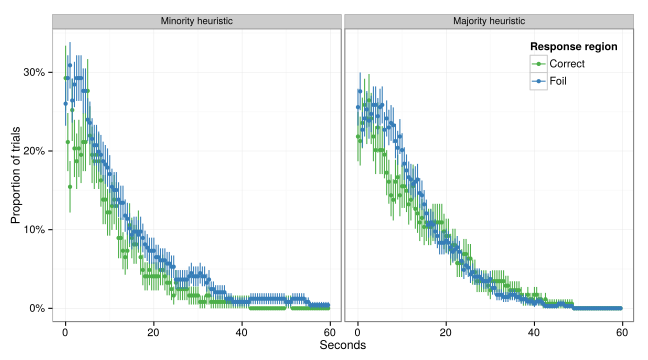
\includegraphics[width=.9\textwidth]{imgs/exp6/heuristic-not-chosen_bias}
  %% \caption[Proportion of cursor in region of other response options
  %%   when heuristic response was given,
  %%   for minority heuristic and majority heuristic particiapants, 
  %%   Experiment 6.]{
  \caption[]{
    Proportion of trials in the region of each option, over time,
    for trials in which the intuitive option was eventually chosen,
    separately for minority heuristic and majority heuristic participants
    (see also Figure~\ref{fig:exp6-heuristic-not-chosen}).
  }
\end{figure}
